\documentclass[11pt]{article}
\usepackage[margin=1in]{geometry}
\usepackage{graphicx}
\usepackage{booktabs}
\usepackage{amsmath,amssymb}
\usepackage[hidelinks]{hyperref}
\usepackage[round]{natbib}
\usepackage{microtype}

\title{What Predicts Correctness in Text-to-SQL?\\ A Selective-Prediction Study}
\author{}
\date{}

\newcommand{\auroc}{\textsc{auroc}}

\begin{document}
\maketitle

\begin{abstract}
Deciding whether to trust a generated SQL query requires an estimate of whether it is correct. We
study which signals provide that estimate on hard multi-table text-to-SQL (BIRD), comparing them on
equal footing with bootstrapped confidence intervals. The black-box statistical signals cluster
together and plateau: string, structural, and execution self-consistency, a schema-relevance score,
and query executability all fall between about $0.61$ and $0.68$ \auroc{}, with string
self-consistency the strongest at $0.675$. White-box log-probability does not beat them ($0.67$). The
signals that move past this ceiling are verification-based: an LLM judge scores from $0.72$
(GPT-4o-mini) to $0.78$ (Claude). Judges from different providers make different errors (their scores
correlate at only $0.43$), so a two-provider ensemble reaches $0.82$ \auroc{} with a well-calibrated
probability (expected calibration error $0.03$), and it supports useful abstention frontiers (for
example, answering $27\%$ of questions at $24\%$ selective risk) where self-consistency offers no
valid low-risk subset. The pattern holds across two generators and two judge providers. We also ask
whether a verifier can be trained. Fine-tuned verifiers, both encoder and generative, reach about
$0.77$--$0.79$ \auroc{} in-distribution but fall to about $0.66$ on unseen schemas, and scaling to
7B, adding schema diversity, distilling a strong judge's rationales, and cross-benchmark training all
fail to close that gap. Cross-schema transfer appears to track model scale and reasoning rather than
fine-tuning. In practice, correctness uncertainty for text-to-SQL lives in reasoning-based signals: a
fine-tuned verifier is a good in-domain tool, while a verifier that generalizes across schemas
currently means a large frozen reasoning model.
\end{abstract}

\section{Introduction}
Text-to-SQL systems are increasingly used where a wrong answer is costly, so deciding when to answer
and when to abstain matters as much as raw accuracy. That decision rests on a calibrated estimate of
whether a generated query is correct. Most uncertainty-quantification (UQ) work for this setting
relies on black-box statistical signals such as sampling agreement \citep{wang2023selfconsistency},
semantic entropy \citep{kuhn2023semantic,farquhar2024semantic}, and structural frequency, which are
appealing because they need no extra model. We ask a direct question: on hard text-to-SQL, which
signals actually predict execution correctness, and by how much?

Our contribution is an execution-grounded comparison, with confidence intervals, of the signals
available to a practitioner, together with the consequences for deployment.
\begin{enumerate}
\item A correctness ceiling for black-box statistical UQ (roughly $0.61$--$0.68$ \auroc{}), shared by
string, structural, and execution self-consistency, by a schema-relevance score, and, once compared
against the strongest of these, by white-box log-probability.
\item Verification moves past the ceiling, with bootstrapped intervals that exclude zero, across two
generators and two judge providers. Judges from different providers make different errors, and an
ensemble of them is the best and best-calibrated correctness signal we obtain ($0.82$ \auroc{},
$0.03$ calibration error).
\item A selective-prediction frontier that the self-consistency baseline cannot match.
\item A study of trained verifiers, which do well in-distribution but fail to transfer across
schemas, separating the in-domain verifier from a universal one.
\end{enumerate}

Our scope is selective prediction rather than generation. We quantify and calibrate correctness to
decide whether to answer or abstain; we do not iterate to improve the query, in contrast with the
self-correcting agents discussed next.

\section{Related work}
\label{sec:related}
Relevant lines of work include self-consistency and sampling-based UQ
\citep{wang2023selfconsistency}, semantic entropy via meaning clustering
\citep{kuhn2023semantic,farquhar2024semantic}, verbalized confidence, conformal and selective
generation \citep{geifman2017selective,angelopoulos2021ltt,angelopoulos2023conformalrisk}, sub-clause
Platt scaling \citep{ramachandran2024calibrating}, and conformal abstention over schema-linking
branch points \citep{somov2025rts}. Schema linking has also been studied with encoder-side graph
models \citep{wang2020ratsql,cao2021lgesql}. LLM-as-judge is widely used for open-ended evaluation;
here we evaluate it specifically as a calibrated correctness predictor for SQL, against black-box
baselines, and we test whether judging can be trained and whether it transfers. We draw data from the
Spider \citep{yu2018spider} and BIRD \citep{li2023bird} benchmarks, and reference Spider~2.0
\citep{lei2025spider2} for context.

A closely related line builds self-correcting or agentic text-to-SQL systems, in which the model
generates a query and then critiques or executes it and regenerates, often over several rounds
\citep{shinn2023reflexion,chen2023selfdebug,pourreza2023dinsql,wang2024macsql}. That work shares a
component with ours, since the critic in such a loop is an LLM verifier much like the judge we study,
but the objective differs: a self-correcting agent uses the critic to drive iteration toward a more
accurate query and reports end-task accuracy. We do not regenerate; we ask how well a signal predicts
correctness so a system can answer or abstain, and we report calibration and risk--coverage rather
than accuracy gains. The two are complementary, because even after self-correction a system emits a
final query and still needs a calibrated estimate of whether to trust it. We check this directly
(Section~\ref{sec:robust}): one round of self-correction barely changes accuracy and produces badly
miscalibrated confidence, so it does not substitute for a calibrated verifier. Typical
self-correction also relies on execution feedback, whereas our verifier reasons over the question,
schema, and SQL without executing the candidate, and we find executability itself uninformative for
correctness.

\section{Setup}
\textit{Benchmark and generation.} We use BIRD \citep{li2023bird}, which has databases with data
dictionaries and external-knowledge ``evidence.'' We generate SQL with GPT-4o-mini ($K=8$ samples
per question, temperature $0.7$, schema and evidence in the prompt) for an 800-question slice across
8 databases, and execute every sample against the real databases to obtain ground-truth correctness.
Modal-query execution accuracy is $0.451$, a hard regime with ample headroom for UQ. A second
generator, GPT-4.1-mini (accuracy $0.522$), is used for a breadth check.

\textit{Signals.} The black-box statistical signals are string self-consistency (the size of the
largest cluster of identical queries among the samples), structural self-consistency (clustering by
canonical query structure), execution self-consistency (clustering by result set), a schema-relevance
score (the average embedding similarity between the question and the tables and columns the query
uses), and query executability (whether the query runs and returns rows). The logic-aware signals are
the mean sequence log-probability of the modal query (white-box) and an LLM verifier shown the
question, evidence, schema, and candidate SQL. The verifiers are GPT-4o-mini and GPT-4o, which report
$P(\text{correct})$ from the YES/NO first-token logits, and Claude-Sonnet-4.6, an
independent-provider judge that reports a verbalized $0$--$100$ probability (Anthropic does not expose
token logprobs).

\textit{Metrics.} We report tie-robust \auroc{} for correctness, with $2{,}000$-sample paired
bootstrap confidence intervals on \auroc{} differences; cross-fit logistic combinations on a parity
split; expected calibration error (ECE) \citep{guo2017calibration}; and risk--coverage with both an
empirical frontier and a distribution-free (Bonferroni-over-grid, $\delta=0.1$) certificate
\citep{angelopoulos2021ltt}. All model outputs are cached; the API experiments are inexpensive (about
\$1.6 total).

\section{Results}

\subsection{The black-box correctness ceiling}
\label{sec:ceiling}
\begin{table}[h]\centering
\begin{tabular}{lr}
\toprule
signal (alone) & \auroc{} for correctness \\
\midrule
string self-consistency (largest identical-query cluster) & 0.675 \\
structural self-consistency (canonical-structure cluster) & 0.619 \\
execution self-consistency (result-set cluster) & 0.613 \\
log-probability (white-box, mean sequence logprob) & 0.669 \\
schema-relevance score & 0.553 \\
executability (runs and returns rows) & 0.500 (chance) \\
\bottomrule
\end{tabular}
\end{table}

The black-box statistical signals plateau between about $0.61$ and $0.68$ \auroc{}, with string
self-consistency the strongest at $0.675$. White-box log-probability does not beat this ceiling
($0.669$; paired difference versus string self-consistency $-0.006$, CI $[-0.028, +0.017]$). It
helped separate confidently wrong queries in earlier single-table settings, but on hard multi-table
data it is no better than sampling agreement. Wrong queries also execute and return rows without
trouble, so executability is uninformative.

\subsection{Verification moves past the ceiling}
\label{sec:verify}
\begin{table}[h]\centering
\begin{tabular}{lrr}
\toprule
signal & \auroc{} & paired $\Delta$ vs string SC (95\% CI) \\
\midrule
log-probability (white-box) & 0.669 & $-0.006\ [-0.028, +0.017]$ (n.s.) \\
LLM verifier (GPT-4o-mini) & 0.724 & $+0.049\ [+0.004, +0.090]$ \\
LLM verifier (GPT-4o) & 0.770 & $+0.095\ [+0.053, +0.138]$ \\
LLM verifier (Claude-Sonnet-4.6) & 0.776 & $+0.101\ [+0.060, +0.141]$ \\
\bottomrule
\end{tabular}
\end{table}

Only the verifiers move past the ceiling, with intervals that exclude zero. The signal that works is
the one not blind to query logic: a model that can reason about whether the aggregation, filters, and
joins answer the question. Notably, combining a strong verifier with self-consistency does not beat
the verifier alone (a cross-fit logistic over GPT-4o plus string self-consistency reaches $0.754$,
below GPT-4o's $0.770$): the gain is the verifier's, not the combination's. The one combination that
does help is across providers (Section~\ref{sec:robust}).

\subsection{Robustness: cross-provider judges, a second generator, and self-correction}
\label{sec:robust}
A verifier from the generator's own family might merely echo it, so we also test an independent
provider. Claude-Sonnet-4.6, judging GPT-4o-mini's SQL, is the strongest single judge ($0.776$ versus
$0.770$), and the two judges' scores correlate at only $r=0.43$, so they make genuinely different
errors. A two-provider ensemble (GPT-4o and Claude) reaches $0.822$ \auroc{} (paired $\Delta$ over
GPT-4o alone $+0.052$, CI $[+0.032, +0.073]$), the strongest correctness signal we obtain, and it is
well-calibrated (ECE $0.031$; Section~\ref{sec:cal}). This rules out a self-agreement artifact and
suggests that combining independent reasoning judges, rather than using one larger judge, is the most
reliable approach. The OpenAI judges use YES/NO logits while Claude reports a verbalized probability;
a method-matched OpenAI verbal judge also clears the ceiling at $0.709$, so the gap is not an
elicitation artifact.

The pattern is not specific to GPT-4o-mini. Regenerating the slice with GPT-4.1-mini (accuracy
$0.522$, a stronger generator) and judging with the same GPT-4o-mini verifier reproduces it.
\begin{table}[h]\centering
\begin{tabular}{lrrrr}
\toprule
generator & accuracy & string SC & verifier & combined $\Delta$ over SC (95\% CI) \\
\midrule
GPT-4o-mini & 0.451 & 0.675 & 0.724 & $+0.059\ [+0.032, +0.087]$ \\
GPT-4.1-mini & 0.522 & 0.641 & 0.677 & $+0.033\ [+0.007, +0.061]$ \\
\bottomrule
\end{tabular}
\end{table}
For both generators, self-consistency sits at the ceiling and the verifier exceeds it, with an
interval that excludes zero. The margin is smaller for GPT-4.1-mini, as expected: there the judge
(GPT-4o-mini) is weaker than the generator and so catches fewer of its subtler errors; a judge at
least as strong as the generator should widen the gap.

\textit{A self-correction baseline.} Self-correction is an alternative way to use a critic, so we run
one reflection round: each modal query is fed back to GPT-4o-mini, which reviews it, revises it if
needed, and reports a confidence. The revision improves execution accuracy only marginally ($0.451$
to $0.468$), and the self-reported confidence is not usable for abstention: it assigns at least $0.9$
confidence to $99\%$ of queries (mean $0.97$), giving \auroc{} $0.637$ and ECE $0.501$. A single
round of self-correction therefore neither closes the accuracy gap nor yields a calibrated trust
signal, so an external verifier remains necessary and abstention is orthogonal to iteration.

\subsection{Can the verifier be trained? In-distribution yes, transfer no}
\label{sec:trained}
We fine-tune verifiers on (question, evidence, schema, SQL) $\rightarrow$ correct, using $6{,}400$
execution-labeled pairs, and evaluate transfer leave-one-database-out (LODO). We compare an encoder
classifier and a generative LLM judge (LoRA), with an un-fine-tuned baseline. Transfer values are
macro-averaged over held-out databases.
\begin{table}[h]\centering
\begin{tabular}{lrr}
\toprule
verifier & in-distribution \auroc{} & transfer (LODO, macro) \\
\midrule
feature classifier (embeddings, logprob, self-consistency) & 0.768 & 0.661 \\
fine-tuned encoder (ModernBERT, full schema) & 0.785 & 0.670 \\
generative judge, 1.5B (LoRA) & 0.766 & 0.659 \\
generative judge, 7B (LoRA) & 0.798 & 0.662 \\
frozen GPT-4o judge (zero-shot) & --- & 0.710 \\
\bottomrule
\end{tabular}
\end{table}

Four findings. First, \emph{fine-tuning works in-distribution}: it lifts the generative judge well
above its zero-shot baseline and reaches the best in-domain numbers (7B at $0.798$). Second, \emph{it
does not transfer}: every fine-tuned verifier, encoder or generative, lands near $0.66$ on unseen
schemas, with the worst results on the most domain-specific databases. The frozen large judge is the
exception; macro-averaged the same way it scores $0.710$ (and $0.770$ pooled over all questions),
above every fine-tuned alternative, and the small base model's near-chance zero-shot transfer shows
why a large model is needed. Third, \emph{nothing closes the gap}: scaling to 7B, adding schema
diversity, distilling a strong judge's rationales, and cross-benchmark training all leave transfer at
about $0.66$--$0.71$ (Appendix~\ref{app:transfer}); only the large frozen reasoning judge reaches
$0.77$. The evidence is consistent with the fine-tuned models relying on schema-specific surface
regularities rather than transferable reasoning: an input ablation of the frozen judge shows it
scores $0.692$ from the question and SQL alone, that adding the schema changes nothing ($0.688$), and
that only the evidence helps ($0.724$), so the frozen judge generalizes by reasoning about the query
rather than by reading schema content. Per database (Figure~\ref{fig:lodo}), the frozen judge leads
on every held-out schema.

Fourth, \emph{the in-domain verifier is useful for deployment}. Trained on a database's own schemas,
it predicts correctness at $0.77$--$0.79$ and is cheap at inference. Used as the abstention score, a
feature classifier with no LLM call at inference gives a risk--coverage frontier competitive with the
frozen GPT-4o judge and far above self-consistency: at a $20\%$ risk target it answers $21\%$ of
questions, against $9\%$ for the frozen judge and $1\%$ for self-consistency (area under the
risk--coverage curve $0.340$, $0.355$, and $0.413$; lower is better). So when a deployment owns its
schemas, a trained verifier is accurate in-domain and the cheaper route to a useful operating point.

\begin{figure}[t]\centering
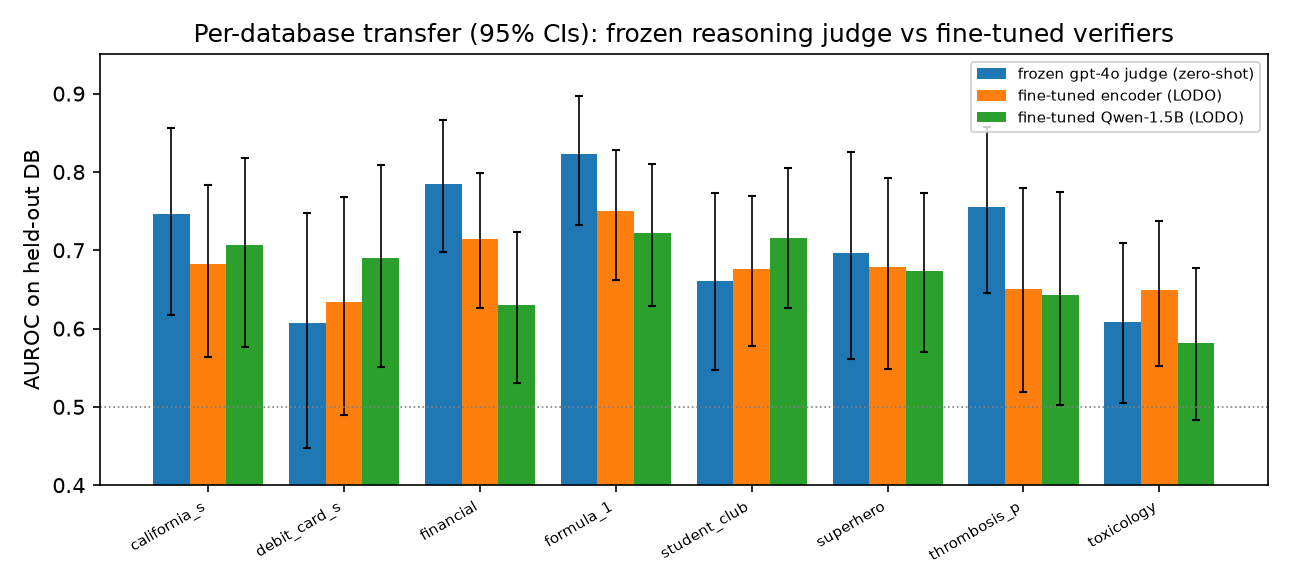
\includegraphics[width=0.48\textwidth]{../figures/paper1_lodo_perdb.png}
\caption{Per-database transfer. The frozen GPT-4o judge leads on every held-out schema, above both
fine-tuned verifiers. Reasoning transfers; fitting captures schema-specific regularities.}
\label{fig:lodo}
\end{figure}

\subsection{Calibration and selective prediction}
\label{sec:cal}
The raw signals are over-confident, while the cross-fit ensemble is well-calibrated and can be used
directly as $P(\text{correct})$ (Figure~\ref{fig:reliab}).
\begin{table}[h]\centering
\begin{tabular}{lrr}
\toprule
score & \auroc{} & ECE \\
\midrule
string self-consistency & 0.675 & 0.212 \\
verifier (GPT-4o, raw $P$) & 0.770 & 0.319 \\
verifier (Claude, raw $P$) & 0.776 & 0.210 \\
two-provider ensemble (cross-fit) & 0.822 & 0.031 \\
\bottomrule
\end{tabular}
\end{table}

For selective prediction we report an empirical risk--coverage frontier (Figure~\ref{fig:rc}), with
the threshold calibrated on a held-out half.
\begin{table}[h]\centering
\begin{tabular}{lll}
\toprule
target risk & self-consistency & all signals \\
\midrule
0.20 & none (no valid subset) & answers 9\% at 14\% risk \\
0.30 & none & answers 27\% at 24\% risk \\
0.40 & none & answers 58\% at 38\% risk \\
\bottomrule
\end{tabular}
\end{table}
Self-consistency cannot form a low-risk subset at any threshold, whereas the logic-aware combination
gives useful empirical frontiers. The distribution-free certificate is conservative under this
regime's low base accuracy ($0.45$): it fires only at the loosest target (all signals at
$\alpha=0.40$, answering $16\%$ at $22\%$ certified risk). A tighter guarantee would need a stronger
generator or more calibration data rather than a better signal, so we treat the empirical frontier as
the practical result and the certificate as a conservative lower bound.

\begin{figure}[t]\centering
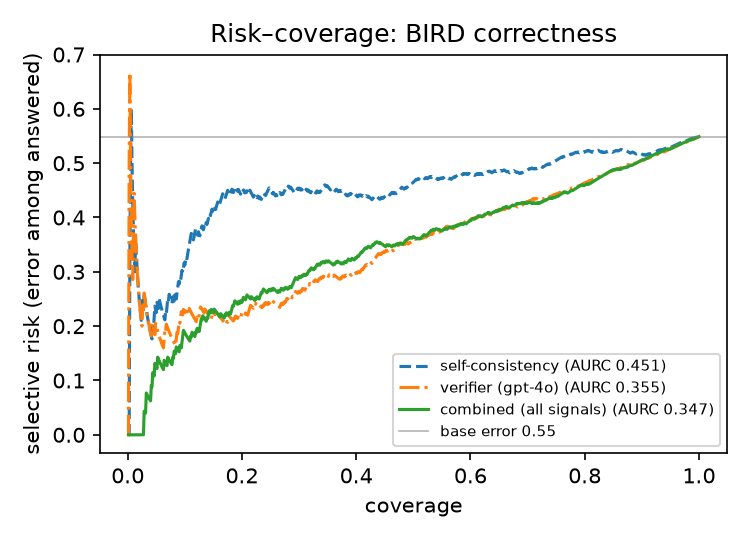
\includegraphics[width=0.48\textwidth]{../figures/paper1_risk_coverage.png}
\hfill
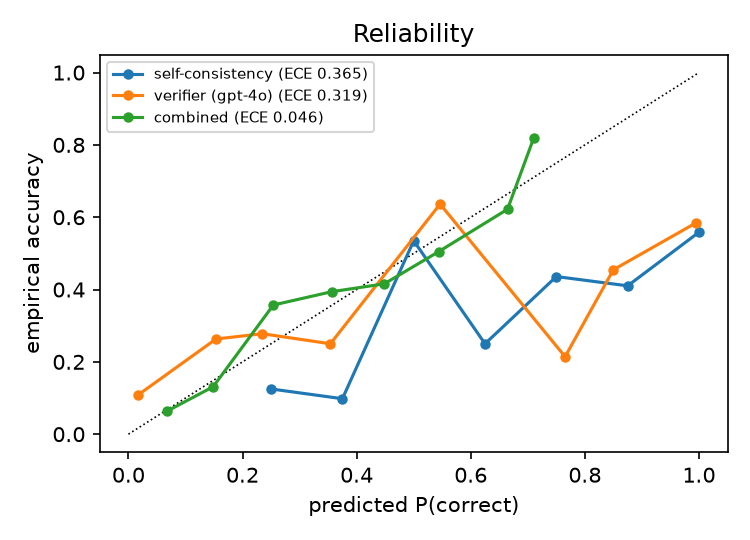
\includegraphics[width=0.48\textwidth]{../figures/paper1_reliability.png}
\caption{Left: risk--coverage, where the ensemble dominates self-consistency. Right: reliability,
where the cross-fit ensemble is calibrated (ECE $0.031$) while the raw signals are over-confident.}
\label{fig:rc}\label{fig:reliab}
\end{figure}

\subsection{Where the errors are: computation, not schema linking}
\label{sec:errors}
Parsing each gold query into structural features and grouping modal correctness by them shows the
errors concentrate in computation and composition, not in schema selection.
\begin{table}[h]\centering
\begin{tabular}{lrr}
\toprule
gold-query feature & accuracy when present & drop vs absent \\
\midrule
arithmetic (ratios, percentages) & 0.277 & $0.210$ \\
nested subquery & 0.280 & $0.183$ \\
CASE expression & 0.286 & $0.180$ \\
GROUP BY & 0.290 & $0.177$ \\
DISTINCT & 0.317 & $0.159$ \\
ORDER BY & 0.331 & $0.151$ \\
multi-table / join & 0.441 & $0.049$ \\
aggregate & 0.451 & $\approx 0$ \\
\bottomrule
\end{tabular}
\end{table}

Join count barely matters (0/1/2/3+ joins: $0.48$/$0.45$/$0.41$/$0.45$), and a logistic over the
features ranks arithmetic, ORDER BY, and DISTINCT as the strongest independent error predictors,
while join and aggregate carry negative coefficients. The benchmark's own difficulty labels line up
as a check (simple $0.544$, moderate $0.332$, challenging $0.287$). The generator largely gets the
tables and columns right and fails on the math, nesting, conditional logic, grouping, and ranking.

This explains the earlier results. A schema-relevance score does not predict correctness
(Section~\ref{sec:ceiling}) because the errors are not in schema selection, and a reasoning verifier
does (Section~\ref{sec:verify}) because catching a wrong ratio or a misgrouped aggregate requires
reasoning about the computation. Consistent with this, the verifier's strongest discrimination is on
the largest error category, arithmetic (\auroc{} $0.813$), and it improves over self-consistency
across query types, including the simpler queries where the model is confidently wrong and
self-consistency is weakest. The one exception is GROUP BY, a small subset where the verifier does not
beat self-consistency.

\section{Discussion}
Correctness uncertainty for text-to-SQL is tractable, but only with signals that engage the query's
logic. The popular black-box statistical signals are a ceiling rather than a solution on hard
multi-table data. Two practical recipes follow. For a fixed deployment, a cheap trained verifier
delivers about $0.78$ at negligible inference cost. For an open setting, a reasoning judge is the
better choice, since a large frozen model already transfers at $0.77$ and combining independent
providers is the most reliable and best-calibrated option.

\section{Limitations}
The generators are within one provider, though we show the effect for two of them, and a judge
stronger than the generator would likely widen the GPT-4.1-mini margin. The certificate is loose under
low base accuracy. Whether a universal trained verifier is possible at much larger scale remains
open; the only verifier that generalizes across schemas in our experiments is the large frozen judge.
Natural extensions include an open-weight generator, a second evaluation benchmark, and a third judge
provider.

\section{Conclusion}
On hard text-to-SQL, what predicts correctness is not sampling agreement, structure, or even
white-box log-probability, all of which plateau between about $0.61$ and $0.68$ \auroc{}. It is
verification: an LLM judge that reasons about whether the query answers the question.
Independent-provider judges make different errors and ensemble to $0.82$ \auroc{} with calibrated
probabilities, enabling empirical abstention the sampling baseline cannot provide. Verifiers can be
trained and are valuable in-domain, but they do not transfer across schemas, so a universal verifier
must generalize by reasoning. The map is the contribution: it indicates which signal to rely on, and
when.

\appendix
\section{Transfer ablations}
\label{app:transfer}
Each row is an attempt to make a fine-tuned verifier transfer to unseen schemas; none closes the gap
to the frozen reasoning judge ($0.710$ macro, $0.770$ pooled). Schema diversity adds Spider's 20
schemas to the training pool (28 in all). Reasoning distillation trains a 1.5B model on a strong
judge's rationales plus the true verdict, versus a verdict-only fine-tune. Cross-benchmark trains on
one benchmark and tests on the other.
\begin{table}[h]\centering
\begin{tabular}{lr}
\toprule
attempt & transfer \auroc{} \\
\midrule
base fine-tune (8 schemas, LODO) & 0.659 \\
+ schema diversity (28 schemas, LODO) & 0.682 \\
scale generative judge to 7B (LODO) & 0.662 \\
reasoning distillation (verdict-only / +reasoning) & 0.653 / 0.564 \\
cross-benchmark (BIRD$\rightarrow$Spider / Spider$\rightarrow$BIRD) & 0.713 / 0.672 \\
\midrule
frozen GPT-4o judge (macro / pooled) & 0.710 / 0.770 \\
\bottomrule
\end{tabular}
\end{table}

\bibliographystyle{plainnat}
\bibliography{references}
\end{document}
